%!Tex Root = ../Tutorat6.tex
% ./Packete.tex
% ./Design.tex
% ./Deklarationen.tex
% ./Aufgabe2.tex
% ./Aufgabe3.tex
% ./Bonus.tex

\section{Task 1}

\setcounter{task}{1}

\begin{frame}[allowframebreaks]{Task 1}{}
  \begin{tasknoinc}
    \centering
    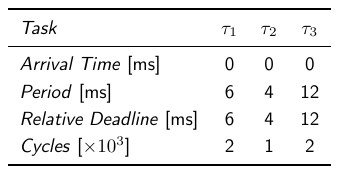
\includegraphics[width=0.4\textwidth]{./figures/task1_tasks.png}

    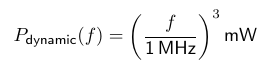
\includegraphics[width=0.4\textwidth]{./figures/task1_power.png}
  \end{tasknoinc}
  \begin{solutionnoinc}
    \centering
    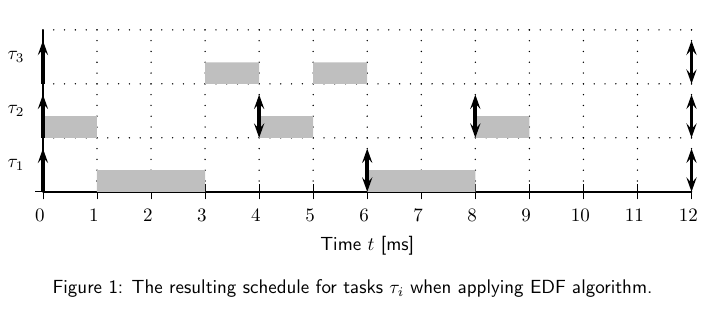
\includegraphics[height=0.6\paperheight]{./figures/task1_schedule.png}
  \end{solutionnoinc}

  \begin{solutionnoinc}
    \centering
    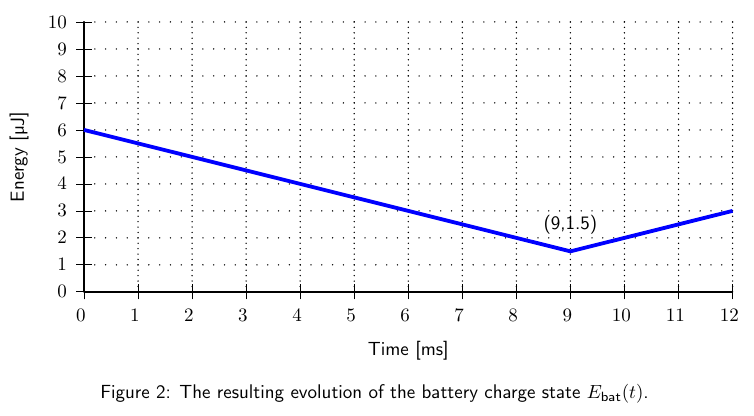
\includegraphics[height=0.6\paperheight]{./figures/task1_energy.png}
  \end{solutionnoinc}
\end{frame}
